\documentclass[tikz]{standalone}
\usetikzlibrary{arrows.meta,positioning,calc}
\usepackage{pgfplots}
\pgfplotsset{compat = newest}

\begin{document}

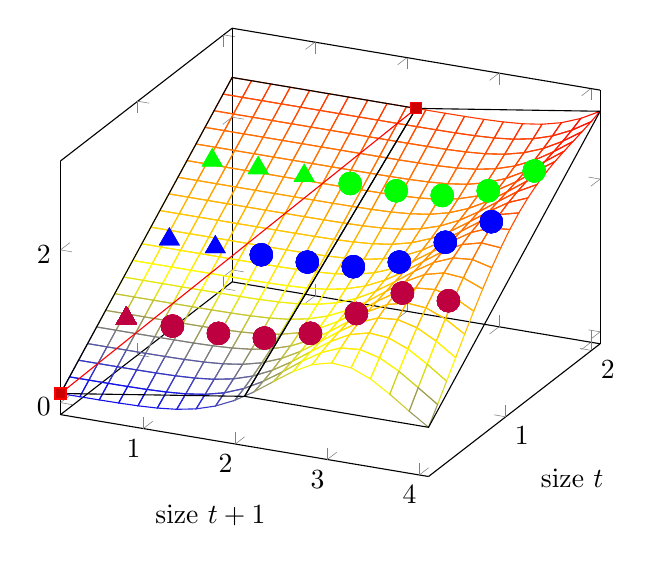
\begin{tikzpicture}[declare function = {f(\x, \y) = exp(-(\x-(\y+3))^2)+\y*1.2;}]
        \begin{axis}[xlabel={size $t+1$}, ylabel={size $t$}]

                \addplot3[mesh, shader=interp, samples=20, domain=0.1:4.1, domain y = 0.1:2.1] {f(x, y)};
                \addplot3 table [z expr = exp(-(x-(y+3))^2) + y*1.2, x = col1,  y = col2, color = black] 
                        {
                        col1 col2
                        0.1 0.1
                        2.1  2.1
                        };
                \addplot3[mesh, shader=interp,samples=3,samples y = 2,domain=0.1:4.1,domain y = 0.1:2.1, color = black] 
                {f(x, y)};
                \addplot3[mark=triangle*,mark size=4pt, color = purple]
                        (0.35,0.6, {exp(-(0.35-(0.6+3))^2) + 0.6 * 1.2});
                \addplot3[domain=0.35:0.85, samples=2, only marks,mark=triangle*,mark size=4pt, color = blue]
                        (x,1.1, {exp(-(x-(1.1+3))^2) + 1.1 * 1.2});
                \addplot3[domain=0.35:1.35, samples=3, only marks,mark=triangle*,mark size=4pt, color = green]
                        (x,1.6,{exp(-(x-(1.6+3))^2) + 1.6 * 1.2});

                \addplot3[domain=0.85:3.85, samples=7, only marks,mark=*,mark size=4pt, color = purple]
                        (x,0.6,{exp(-(x-(0.6+3))^2) + 0.6 * 1.2});
                \addplot3[domain=1.35:3.85, samples=6, only marks,mark=*,mark size=4pt, color = blue]
                        (x,1.1, {exp(-(x-(1.1+3))^2) + 1.1 * 1.2});
                \addplot3[domain=1.85:3.85, samples=5, only marks,mark=*,mark size=4pt, color = green]
                        (x,1.6, {exp(-(x-(1.6+3))^2) + 1.6 * 1.2} );


                % line not working, don't know why
                % \addplot3[domain=1.85:3.85, samples=5, only marks,mark=*,mark size=4pt, color = green]
                        % (x,1.6, {f(x, 1.6)} );

        \end{axis}
\end{tikzpicture}

\end{document}